%In Figure 2~\ref{process} the three steps of the conduction phase. As can be seen, in Step 1, we identified primary studies in the digital libraries. The digital libraries Scopus has returned more primary studies than the others(262), i.e., IEEE, ACM and Springer have returned 215, 202 and 127, respectively. Possibly, this came about because this digital library indexes studies of others libraries, such as IEEE and Springer. Summing up, we have gotten 802 primary studies in the Step 1. In the Step 2 we have selected the primary studies by means of reading the titles and abstracts and the application of the inclusion and exclusion criteria. As a result, we have gotten a total of 124 primary studies that were read entirely, so the upshot obtained in the Step 3 were 62. Among these 62 primary studies we have identified 18 mining techniques for crosscutting concern. Therefore, each included primary study was assigned to one or more techniques.
%
%\begin{figure}[!h]
%\centering
%  % Requires \usepackage{graphicx}
%  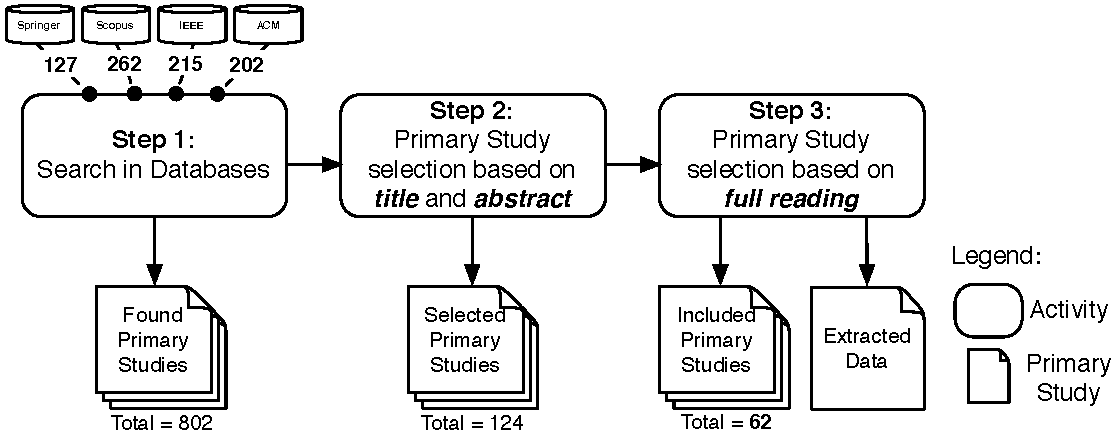
\includegraphics[scale=0.4]{figuras/process_conducted}
%\caption{Papers retrieved from each electronic database, total of candidate studies and the final set.}
%\label{process}
%\end{figure} 

In this phase, firstly we identified primary studies in the digital libraries. The digital libraries Scopus has returned more primary studies than the others (262), i.e., IEEE, ACM and Springer have returned 215, 202 and 127, respectively. Possibly, this came about because this digital library indexes studies of others libraries, such as IEEE and Springer. Summing up, we have gotten 802 primary studies. Afterwards we have selected the primary studies by means of reading the titles and abstracts and the application of the inclusion and exclusion criteria. As a result, we have gotten a total of 124 primary studies that were read entirely, so the upshot obtained were 62 studies. 

Among these 62 primary studies we have identified 18 mining techniques for crosscutting concern. Therefore, each included primary study was assigned to one or more techniques. In the following we outline each of the techniques: 

\begin{itemize}

\item \textit{Execution Patterns (EP)}: During program execution, program traces are generated, which reflect the run-time behavior of a software system. These traces are then investigated for recurring execution patterns. In~\cite{Breu:2004:AMU:1025115.1025235} the authors introduce the notion of execution relations between method invocation. In other words, the basic idea of EP is to observer run-time behavior of software system and to extract information from the execution of the programs. As example, consider the Figure X, wherein that capitals represent methods names. According to Breu and Krinke~\cite{Breu:2004:AMU:1025115.1025235} exist four different execution relations, they are: (\textit{i}) outside-before, see Figure X, where B is called before A, (\textit{ii}) outside-after, where A is called after B, see Figure X, (\textit{iii}) inside-first, G is the first call in C and (\textit{iv}) inside-last, H is the last call in C. 


%This technique analyses program traces reflecting the run-time behavior of a system in search of recurring execution patterns. Thus, their mining algorithm discovers concern candidates based on recurring patterns of method invocations~\cite{Breu:2004:AMU:1025115.1025235}.

\item \textit{Dynamic Analysis (DA)}: DA is the analysis of the properties of a running program, whereas to static analysis, which examines a program's text to derive properties that hold for all executions, DA derives properties that hold for one or more executions by examination of the running program. 
While DA cannot prove that a program satisfies a particular property, it can detect violation of properties as well as provide useful information to programmers about the behavior of their programs. 
The usefulness of DA supplies from two of its essential characteristic:
\begin{itemize}

\item Precision of information: DA typically involves instrumenting a program to examine or record certain aspects of its run-time state. This instrumentation can be tuned to collect precisely the information needed to address a particular problem. For example, to analyze the shape of data structures created by a program (lists, trees, dags, etc.), an instrumentation tool can be created to record the linkages among heap-allocated storage cells;

\item Dependence on program inputs: the very thing makes DA incomplete also supplies a powerful mechanism for relating program inputs and outputs to program behavior. With DA it is straightforward to relate changes in program inputs to changes in internal program behavior and program outputs, since all are directly observable and linked by the program execution. Viewed in this light, dynamic and static analysis might be better termed ``input-centric'' and ``program-centric'' analysis, respectively.
 

\end{itemize}

Dynamic and static analyses are complementary techniques in a number of dimensions, them are: 

\begin{itemize}

\item Completeness: In general, dynamic analyses generate ``dynamic program invariants'', properties which are true for the observed set of execution. Static analysis can help determine or not these dynamic ``invariants'' truly are invariants over all program executions. In the cases where the dynamic and static analyses disagree, there are two possibilities: (\textit{i}) the dynamic analysis is in error because it did not cover a sufficient number of executions, (\textit{ii}) the static analysis is in error because it analyzed infeasible path;

\item Scope: Because dynamic analysis examines one very long program path, it has the potential to discover semantic dependencies between program entities widely separated in the path. Static analysis typically is restricted in the scope of a program it can analyze and efficiently, and may have troubles discovering such ``dependencies at a distance''.

\item Precision:  DA has the benefit of examining the concrete domain of the program execution. In other hands, static analysis must abstract over this domain in order to ensure termination of the analysis, thus, it can lose information. 

\end{itemize}

%DA deals with task scenarios that formulate the user-system interactions in an informal or semi-formal manner. 
%DA with its suitability in extraction system functionality has several challenges compared to the Static Analysis (SA): 
%(\textit{i}) a SA usually generates a complete set of software facts through parsing or lexical analysis of the source code based on a domain model, 
%whereas in DA only a small subset of the possible dynamic traces are extracted, 
%(\textit{ii}) obtaining meaningful knowledge from the extracted execution traces is a difficult task that affects the applicability of the DA, 
%(\textit{iii}) the large sizes of the execution traces that are caused by program constructs such as loops and recursions may disfunction the whole dynamic analysis. 
In the context of discovering possible concerns DA applies FCA\footnote{FCA is a mathematical theory of data analysis which describe relationship between a particular set of objects and a particular set of attributes~\cite{PrissFCA}} to get execution traces.
In other words, the obtained execution traces are analyzed using FCA for identifying methods and classes.  
%In order to discover possible concerns DA applies formal concept analysis (FCA) to get execution traces. 
%A version of the system is executed on a number of use cases. 
%The obtained execution traces are analyzed using FCA for identifying methods and classes. 
Thus, methods belonging to more than one class may indicate presence of scattering code. 
If different methods from same class are specific to more than one use-case may indicate presence of tangling code~\cite{Ceccato:2008:ASM:1545010.1545380}.

\item \textit{Identifier Analysis (IA)}: This technique performs an identifier analysis using FCA algorithm. The assumption behind this approach is that relevant concerns in the source code are reflected by the use of naming conventions in the classes and methods of the system. As input to FCA algorithm, the classes and methods are used as objects and substrings generated from the classes and methods names are used as attributes. The resulting concepts consists out of maximal groups of classes and methods which share a maximal number of substrings~\cite{Tourwe:2004:MAV:1018444.1022149}.

\item \textit{Language Clues (LC)}: The approach uses natural language processing for mining crosscutting concern. The input is a collection of words from the source code and the output, chains of words which are semantically strongly related calculated with an algorithm. In order to mine for crosscutting concerns, they apply the chaining algorithm to the comments, method names, field names and class names of the system. A manual inspection to the resulting chains is needed in order to select possible concerns~\cite{Shepherd:2005:ULC:1083125.1083129}.

\item \textit{Method Clustering (MC)}: This technique starts by putting each method in a separate cluster and then, recursively, merges clusters by similarities in method names~\cite{Bernardi2009CTI}. 

\item \textit{Call Clustering (CC)}: This technique starts from the assumption that if the same methods are called frequently from within different modules, then, they are closely related and must be clustered~\cite{Danfeng}.


\item \textit{Fan-In analysis (FI)}: It is an approach that involves looking for methods that are called from many different call sites and whose functionality is needed across different methods, potentially spread over many classes and packages. 
FI is a semi-automated process consisting of three steps. Firstly, the method with the highest fan-in values need to be identified. Secondly, one have to filter out methods that may have a high fan-in but for which it is unlikely that there is a systematic pattern in their usage that could be exploited in an aspect solution. Common examples are getters and setters, and utility methods as well. Thirdly, the call sites of the high fan-in methods need to be inspected to determine if the method in questions does indeed implement crosscutting functionality. The last step is the most labor intensive, and it is based on an analysis of recurring patterns in, for example, the call sites of the high fan-in method~\cite{Marin:2007:ICC:1314493.1314496}.
%Through fan-in metric, this approach can measure the number of methods that call some other methods.
High fan-in metric values may indicate presence of a crosscutting concern~\cite{Danfeng}.

\item \textit{AST-Based Clone Detection (ACD)}: This technique takes the Abstract Syntax Tree (AST) of the source code into account. The output is a number of clone classes, i.e. groups of code fragments which are considered to be clones of each other~\cite{Bruntink2005}.

\item \textit{Token-Based Clone Detection (TCD)}: This technique is based on lexical analysis of the source code. The output is a number of clone classes, i.e., groups of code fragments which are considered to be clones of each other~\cite{Bruntink2005}.

\item \textit{History Based (HB)}: This technique intends to discover crosscutting concerns by analyzing the changes made in the source code along the time by using software repositories like revision control systems, files and databases~\cite{Mulder:2010:ICC:1862372.1862381}.

\item \textit{Information Retrieval (IR)}: This technique tries to identify concerns. It is based on the similarity between terms used in the concern descriptions and in the program elements, e.g., element names, variable names. The results are ranked and a manual inspection is performed~\cite{Eaddy:2008:CTR:1437898.1438590}.

\item \textit{Parser-Based (PB)}: This technique performs a lexical or syntactic analysis of the source code to locate crosscutting concerns. It is based on the premise that code fragments which share concerns are likely to refer to readily identifiable shared entities such as identifiers and libraries~\cite{Griswold}.

\item \textit{PrefixSpan (PS)}: It is a data mining technique used to identify coding patterns in source code. Each method in a program is translated to a sequence that comprises method call elements and control elements. The algorithm searches for repetitive subsequences that could form a pattern~\cite{Ishio:2008:MCP:1447565.1448040}.

\item \textit{Concern-Peers (CP)}: This technique identifies certain groups of code units that potentially share some crosscutting concerns. These code units, called concern peers, are detected based on their similar interactions (similar calling relations in similar contexts, either internally or externally). The algorithm scan for candidates, i.e., methods with similar code and names, then scan for peers and rank it to recommend possible concerns~\cite{Nguyen2011}. 

\item \textit{Method Call Tree (MCT)}: It uses method call tree to generate method call traces. These traces are then investigated for recurring method patterns based on different constraints, such as, the requirement that the patterns exist in always the same composition and in different calling contexts in the method call trace~\cite{Qu:2007:AMU:1262690.1262897}.

\item \textit{Data-Flow Concern Identification (DF)}: It is a semiautomated approach for concern identification specifically designed to support software understanding. It starts from a set of related variables and uses static dataflow information to determine the concern skeleton, a data-oriented abstraction of a concern~\cite{Trifu:2008:UDI:1545010.1545363}.

\item \textit{Random Walks (RW)}: A random walk is a mathematical formalization of a trajectory that consists of taking successive random steps. This technique performs a random walks on the coupling graphs extracted from the program sources. The algorithm reflects the degrees of ``popularity and significance" for each of the program elements on the coupling graphs. Filtering techniques, exploiting both types of ranks, are applied to produce a final list of candidate crosscutting concerns~\cite{CharlesZhang2011}.

\item \textit{Model-Driven (MD)}: This technique is a model driven approach for concern mining and their separation, which automatically identifies desirable candidate concerns, without requiring input from the user. The concern miner acts as a model transformer converting the source code to a concern-oriented model~\cite{Nora}.

\end{itemize}

The taxonomy proposed by Kellens et al.~\cite{Kellens}, takes into account 3 dimensions: \textit{(i)} static or dynamic analysis; if the technique does a static analysis of the code or dynamic information which is obtained by executing the program or both. \textit{(ii)} Token-Based or structural/behavioral analysis; lexical analysis like sequences of characters, regular expression or abstract syntax trees, type information, message sends, etc. \textit{(iii)} Granularity: The level of granularity of the technique, method level or more fine-grained. 

In this context, we have extended the taxonomy proposed by Kellens et al.~\cite{Kellens} by means of adding the new identified mining techniques. In Figure~\ref{taxonomy}, it is depicted our extended taxonomy. The small rectangles in the middle of the figure represent all of the techniques: the previous ones, proposed by Kellens et al.~\cite{Kellens} and the new ones proposed by us, marked with an asterisk in Figure~\ref{taxonomy}. More specifically, from the 18 techniques identified herein, 7 of them are new and were added to the taxonomy. The new techniques are: PrefixSpan, Information Retrieval, Dataflow, Model-Driven, Random Walks, History-Based, Concern Peers. The details on each of the identified new techniques and algorithms are outside the scope of this paper. Also, the fact of adding new techniques asked for the inclusion of new algorithms in the taxonomy as well. So, we added four algorithms, they are: Vector Space Indexing, Frecuent Itemset, Concern Model, Peer Detection. 
Finally, a new granularity level was added because the history-based technique can search for crosscutting concerns into source code repositories. 

%We argue that this taxonomy could serve as an initial roadmap for crosscutting concern researchers. Moreover, it is could be relevant for tool developers who might have knowledge about the best aspect indicators to use or who may have certain demands about the granularity of the results.



 %This taxonomy could serve as an initial roadmap to crosscutting concern miners and researchers. Each of the 18 mining techniques for crosscutting concern identified are represented by a small rectangle. The six larger rectangles distinguish  `static' from `dynamic' techniques, and `method-level' techniques from techniques which report both `method fragment' and `file-level' as seeds. Finally, the two rounded rectangles on the left partition represent techniques which use `token-based' and `structural/behavioral' ones.

\begin{figure}
\centering
  % Requires \usepackage{graphicx}
  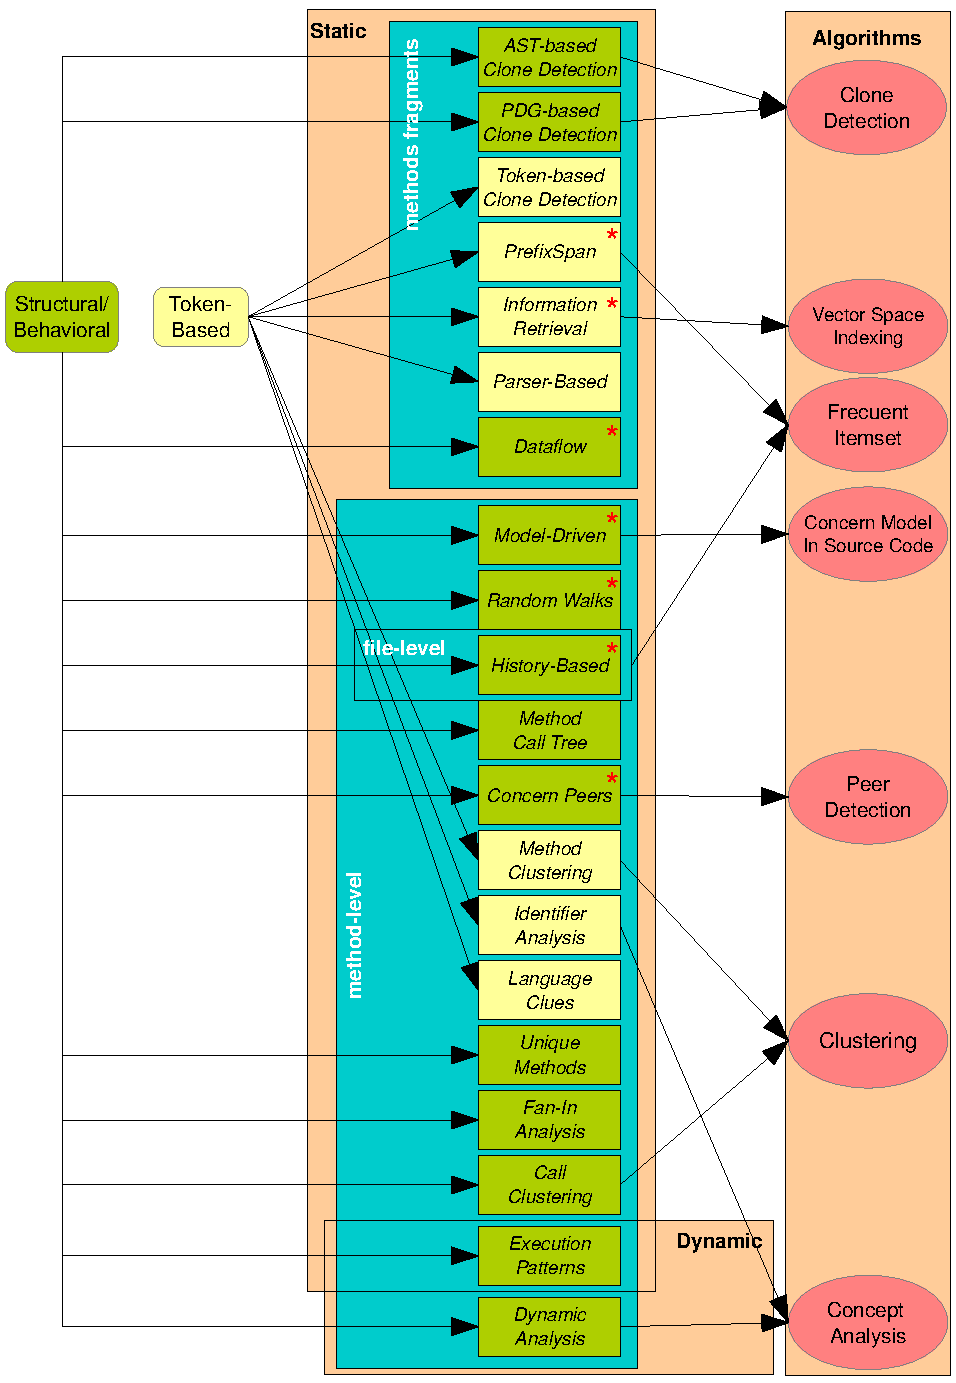
\includegraphics[width=8cm, height=13cm]{figuras/taxonomy}
\caption{The Extended Taxonomy (Adapted from \textit{Kellens et al.}~\cite{Kellens}).}
\label{taxonomy}
\end{figure} 